\section{Four 4-transpositions}

\begin{lemma}
  \label{proof-4-1}
  There is a single sggi of rank 4 over $A_{11}$ composed by 4-transposition. This sggi is represented in the Appendix~\ref{rank4-4-4transpositions} (p. \pageref{rank4-4-4transpositions}).
\end{lemma}

\begin{proof}
  Here is the common graph with the involutions $\rho_1$.

  \begin{figure}[H]
    \begin{center}
      \begin{tikzpicture}[scale=.8]

        \begin{scope}[every node/.style={circle,draw, transform shape}]
          \node (1)  at (0,0)  {};
          \node (2)  at (2,0)  {};
          \node (3)  at (4,0)  {};
          \node (4)  at (6,0)  {};
          \node (5)  at (8,0)  {};
          \node (6)  at (10,0)  {};
          \node (7)  at (12,0)  {};
          \node (8)  at (14,0)  {};
          \node (9)  at (16,0)  {};
          \node (10) at (18,0)  {};
          \node (11) at (20,0) {};
        \end{scope}

        \begin{scope}[every node/.style={fill=white, transform shape}]

          \begin{scope}[every edge/.style={draw}]
            \path (1)  edge node {$1$} (2);
            \path (3)  edge node {$1$} (4);
            \path (5)  edge node {$1$} (6);
            \path (7)  edge node {$1$} (8);
          \end{scope}
        \end{scope}

      \end{tikzpicture}
      \caption{}
    \end{center}
  \end{figure}

  \paragraph{}
  By Lemma~\ref{rank-4-3-patterns}, a double edge and a link between two fixed points must be built for $\rho_1$ and $\rho_3$.

  \begin{figure}[H]
    \begin{center}
      \begin{tikzpicture}[scale=.8]

        \begin{scope}[every node/.style={circle,draw, transform shape}]
          \node (1)  at (0,2)  {};
          \node (2)  at (0,0)  {};
          \node (3)  at (2,2)  {};
          \node (4)  at (2,0)  {};
          \node (5)  at (4,0)  {};
          \node (6)  at (6,0)  {};
          \node (7)  at (8,0)  {};
          \node (8)  at (10,0)  {};
          \node (9)  at (14,0) {};
          \node (10) at (12,0) {};
          \node (11) at (16,0) {};
        \end{scope}

        \begin{scope}[every node/.style={fill=white, transform shape}]

          \begin{scope}[every edge/.style={draw}]
            \path (1)  edge node {$1$} (2);
            \path (3)  edge node {$1$} (4);
            \path (5)  edge[bend left=30] node {$1$} (6);
            \path (7)  edge node {$1$} (8);
            \path (1)  edge node {$3$} (3);
            \path (2)  edge node {$3$} (4);
            \path (5)  edge[bend right=30] node {$3$} (6);
            \path (9)  edge node {$3$} (10);
          \end{scope}
        \end{scope}

      \end{tikzpicture}
      \caption{}
    \end{center}
  \end{figure}

  \paragraph{}
  Also by Lemma~\ref{rank-4-3-patterns}, $\rho_0$ and $\rho_2$ must form the same patterns. Thus there are at least two alternating squares. There are some possibilities for the relations between both squares.

  \paragraph{}
  \textbf{All vertices shared}

  \paragraph{}
  If all vertices are shared, then the square cannot be connected.

  \paragraph{}
  \textbf{Two vertices shared}

  \paragraph{}
  In this case, there is a single possible graph by Proposition~\ref{linear-pattern}:

  \begin{figure}[H]
    \begin{center}
      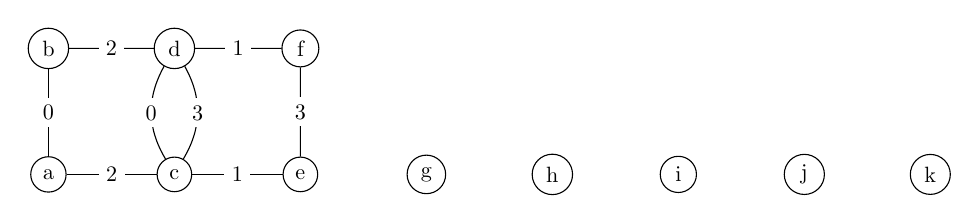
\begin{tikzpicture}[scale=.8]

        \begin{scope}[every node/.style={circle,draw, transform shape}]
          \node (1)  at (0,0)  {a};
          \node (2)  at (0,2)  {b};
          \node (3)  at (2,0)  {c};
          \node (4)  at (2,2)  {d};
          \node (5)  at (4,0)  {e};
          \node (6)  at (4,2)  {f};
          \node (7)  at (6,0)  {g};
          \node (8)  at (8,0)  {h};
          \node (9)  at (10,0) {i};
          \node (10) at (12,0) {j};
          \node (11) at (14,0) {k};
        \end{scope}

        \begin{scope}[every node/.style={fill=white, transform shape}]

          \begin{scope}[every edge/.style={draw}]
            \path (1)  edge node {$0$} (2);
            \path (3)  edge[bend left=30] node {$0$} (4);
            \path (3)  edge node {$1$} (5);
            \path (4)  edge node {$1$} (6);
            \path (1)  edge node {$2$} (3);
            \path (2)  edge node {$2$} (4);
            \path (3)  edge[bend right=30] node {$3$} (4);
            \path (5)  edge node {$3$} (6);
          \end{scope}
        \end{scope}

      \end{tikzpicture}
      \caption{}
    \end{center}
  \end{figure}

  \paragraph{}
  If the sequence is extended, the possible adjacent squares are $[\rho_0,\rho_3]$, $[\rho_2, \rho_3]$ or $[\rho_0, \rho_2]$. In all cases, it uses $\rho_1$ or $\rho_2$ edges and thus some $\rho_0$ or $\rho_3$ edge must be placed in alternating squares but there are not enough points.

  \paragraph{}
  If the sequence is not extended, one $\rho_2$ edge must connect the square to a fixed point (up to duality).

  \begin{figure}[H]
    \begin{center}
      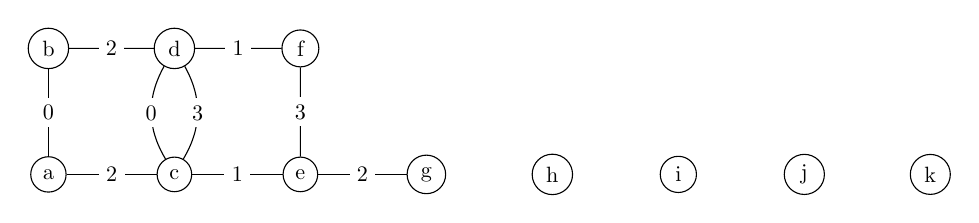
\begin{tikzpicture}[scale=.8]

        \begin{scope}[every node/.style={circle,draw, transform shape}]
          \node (1)  at (0,0)  {a};
          \node (2)  at (0,2)  {b};
          \node (3)  at (2,0)  {c};
          \node (4)  at (2,2)  {d};
          \node (5)  at (4,0)  {e};
          \node (6)  at (4,2)  {f};
          \node (7)  at (6,0)  {g};
          \node (8)  at (8,0)  {h};
          \node (9)  at (10,0) {i};
          \node (10) at (12,0) {j};
          \node (11) at (14,0) {k};
        \end{scope}

        \begin{scope}[every node/.style={fill=white, transform shape}]

          \begin{scope}[every edge/.style={draw}]
            \path (1)  edge node {$0$} (2);
            \path (3)  edge[bend left=30] node {$0$} (4);
            \path (3)  edge node {$1$} (5);
            \path (4)  edge node {$1$} (6);
            \path (1)  edge node {$2$} (3);
            \path (2)  edge node {$2$} (4);
            \path (5)  edge node {$2$} (7);
            \path (3)  edge[bend right=30] node {$3$} (4);
            \path (5)  edge node {$3$} (6);
          \end{scope}
        \end{scope}

      \end{tikzpicture}
      \caption{}
    \end{center}
  \end{figure}

  \paragraph{}
  Now, there are four remaining points. We can build an alternating square. This square must be $[\rho_1, \rho_3]$ but then there are two $\rho_0$ edges and no $\rho_1$. No new alternating square can be built because there are not enough points.

  \paragraph{}
  No $\rho_0$ edge can be placed inside existing square and there are two remaining $\rho_0$ edges for one $\rho_1$ and by Proposition~\ref{rho0atEnd} the graph will never be completed.

  \paragraph{}
  \textbf{No share}

  \paragraph{}
  In this case, both squares already use eight points.

  \begin{figure}[H]
    \begin{center}
      \begin{tikzpicture}[scale=.8]

        \begin{scope}[every node/.style={circle,draw, transform shape}]
          \node (1)  at (0,2)  {};
          \node (2)  at (0,0)  {};
          \node (3)  at (2,2)  {};
          \node (4)  at (2,0)  {};
          \node (5)  at (4,0)  {};
          \node (6)  at (6,0)  {};
          \node (7)  at (8,0)  {};
          \node (8)  at (10,0) {};
          \node (9)  at (10,2) {};
          \node (10) at (12,0) {};
          \node (11) at (12,2) {};
        \end{scope}

        \begin{scope}[every node/.style={fill=white, transform shape}]

          \begin{scope}[every edge/.style={draw}]
            \path (1)  edge node {$0$} (2);
            \path (3)  edge node {$0$} (4);
            \path (8)  edge node {$1$} (10);
            \path (9)  edge node {$1$} (11);
            \path (1)  edge node {$2$} (3);
            \path (2)  edge node {$2$} (4);
            \path (8)  edge node {$3$} (9);
            \path (10) edge node {$3$} (11);
          \end{scope}
        \end{scope}

      \end{tikzpicture}
      \caption{}
    \end{center}
  \end{figure}

  \paragraph{}
  If a square is extended in a sequence, this sequence cannot have a length bigger than two because there are not enough points. Suppose that this square is $[\rho_0, \rho_2]$, the new square must left one $\rho_1$ and one $\rho_3$ edges to link the two squares together. Thus the new square must be $[\rho_0, \rho_3]$.

  \begin{figure}[H]
    \begin{center}
      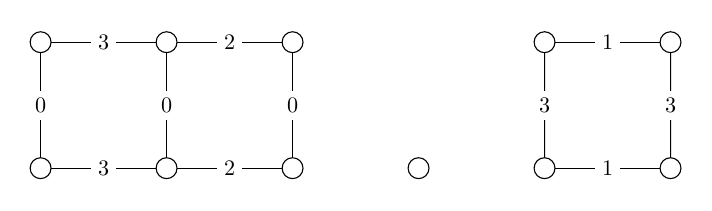
\begin{tikzpicture}[scale=.8]

        \begin{scope}[every node/.style={circle,draw, transform shape}]
          \node (1)  at (0,2)  {};
          \node (2)  at (0,0)  {};
          \node (3)  at (2,2)  {};
          \node (4)  at (2,0)  {};
          \node (5)  at (-2,0) {};
          \node (6)  at (-2,2) {};
          \node (7)  at (4,0)  {};
          \node (8)  at (6,0)  {};
          \node (9)  at (6,2)  {};
          \node (10) at (8,0)  {};
          \node (11) at (8,2)  {};
        \end{scope}

        \begin{scope}[every node/.style={fill=white, transform shape}]

          \begin{scope}[every edge/.style={draw}]
            \path (1)  edge node {$0$} (2);
            \path (3)  edge node {$0$} (4);
            \path (5)  edge node {$0$} (6);
            \path (8)  edge node {$1$} (10);
            \path (9)  edge node {$1$} (11);
            \path (1)  edge node {$2$} (3);
            \path (2)  edge node {$2$} (4);
            \path (1)  edge node {$3$} (6);
            \path (2)  edge node {$3$} (5);
            \path (8)  edge node {$3$} (9);
            \path (10) edge node {$3$} (11);
          \end{scope}
        \end{scope}

      \end{tikzpicture}
      \caption{}
    \end{center}
  \end{figure}

  \paragraph{}
  Now we must connect the two squares together using one $\rho_1$ edge and one $\rho_2$ edge.

  \begin{figure}[H]
    \begin{center}
      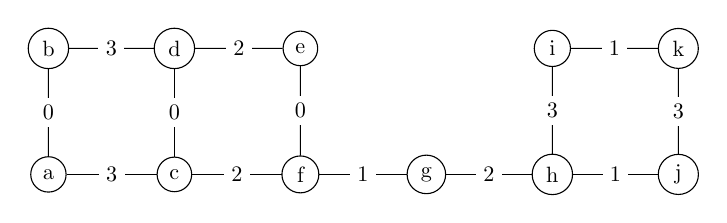
\begin{tikzpicture}[scale=.8]

        \begin{scope}[every node/.style={circle,draw, transform shape}]
          \node (1)  at (0,2)  {d};
          \node (2)  at (0,0)  {c};
          \node (3)  at (2,2)  {e};
          \node (4)  at (2,0)  {f};
          \node (5)  at (-2,0) {a};
          \node (6)  at (-2,2) {b};
          \node (7)  at (4,0)  {g};
          \node (8)  at (6,0)  {h};
          \node (9)  at (6,2)  {i};
          \node (10) at (8,0)  {j};
          \node (11) at (8,2)  {k};
        \end{scope}

        \begin{scope}[every node/.style={fill=white, transform shape}]

          \begin{scope}[every edge/.style={draw}]
            \path (1)  edge node {$0$} (2);
            \path (3)  edge node {$0$} (4);
            \path (5)  edge node {$0$} (6);
            \path (8)  edge node {$1$} (10);
            \path (9)  edge node {$1$} (11);
            \path (4)  edge node {$1$} (7);
            \path (1)  edge node {$2$} (3);
            \path (2)  edge node {$2$} (4);
            \path (7)  edge node {$2$} (8);
            \path (1)  edge node {$3$} (6);
            \path (2)  edge node {$3$} (5);
            \path (8)  edge node {$3$} (9);
            \path (10) edge node {$3$} (11);
          \end{scope}
        \end{scope}

      \end{tikzpicture}
      \caption{}
    \end{center}
  \end{figure}

  \paragraph{}
  The last $\rho_0$ edge must be placed on $(j,k)$. But there are no available positions for the last $\rho_1$ edge. Thus this does not lead to any valid sggi.

  \paragraph{}
  Thus none of the two alternating squares can be extended and they must be linked by a single edge.

  \begin{figure}[H]
    \begin{center}
      \begin{tikzpicture}[scale=.8]

        \begin{scope}[every node/.style={circle,draw, transform shape}]
          \node (1)  at (0,2)  {};
          \node (2)  at (0,0)  {};
          \node (3)  at (2,2)  {};
          \node (4)  at (2,0)  {};
          \node (5)  at (4,0)  {};
          \node (6)  at (6,0)  {};
          \node (7)  at (8,0)  {};
          \node (8)  at (10,0) {};
          \node (9)  at (10,2) {};
          \node (10) at (12,0) {};
          \node (11) at (12,2) {};
        \end{scope}

        \begin{scope}[every node/.style={fill=white, transform shape}]

          \begin{scope}[every edge/.style={draw}]
            \path (1)  edge node {$0$} (2);
            \path (3)  edge node {$0$} (4);
            \path (4)  edge node {$1$} (5);
            \path (8)  edge node {$1$} (10);
            \path (9)  edge node {$1$} (11);
            \path (1)  edge node {$2$} (3);
            \path (2)  edge node {$2$} (4);
            \path (7)  edge node {$2$} (8);
            \path (8)  edge node {$3$} (9);
            \path (10) edge node {$3$} (11);
          \end{scope}
        \end{scope}

      \end{tikzpicture}
      \caption{}
    \end{center}
  \end{figure}

  \paragraph{}
  Then there are three possibilities to link both components: a chain $\rho_0, \rho_1$, a chain $\rho_2, \rho_1$ or a chain $\rho_3, \rho_1$. The last case is the dual of the first case.

  \begin{figure}[H]
    \begin{center}
      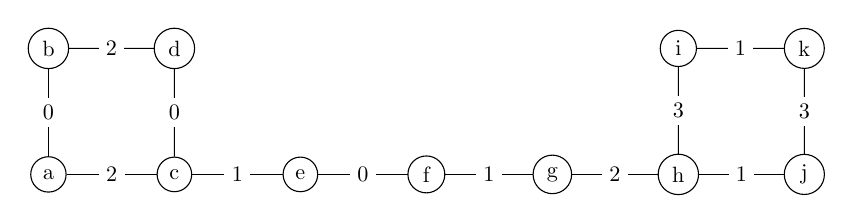
\begin{tikzpicture}[scale=.8]

        \begin{scope}[every node/.style={circle,draw, transform shape}]
          \node (1)  at (0,2)  {b};
          \node (2)  at (0,0)  {a};
          \node (3)  at (2,2)  {d};
          \node (4)  at (2,0)  {c};
          \node (5)  at (4,0)  {e};
          \node (6)  at (6,0)  {f};
          \node (7)  at (8,0)  {g};
          \node (8)  at (10,0) {h};
          \node (9)  at (10,2) {i};
          \node (10) at (12,0) {j};
          \node (11) at (12,2) {k};
        \end{scope}

        \begin{scope}[every node/.style={fill=white, transform shape}]

          \begin{scope}[every edge/.style={draw}]
            \path (1)  edge node {$0$} (2);
            \path (3)  edge node {$0$} (4);
            \path (5)  edge node {$0$} (6);
            \path (4)  edge node {$1$} (5);
            \path (6)  edge node {$1$} (7);
            \path (8)  edge node {$1$} (10);
            \path (9)  edge node {$1$} (11);
            \path (1)  edge node {$2$} (3);
            \path (2)  edge node {$2$} (4);
            \path (7)  edge node {$2$} (8);
            \path (8)  edge node {$3$} (9);
            \path (10) edge node {$3$} (11);
          \end{scope}
        \end{scope}

      \end{tikzpicture}
      \caption{}
    \end{center}
  \end{figure}

  \begin{figure}[H]
    \begin{center}
      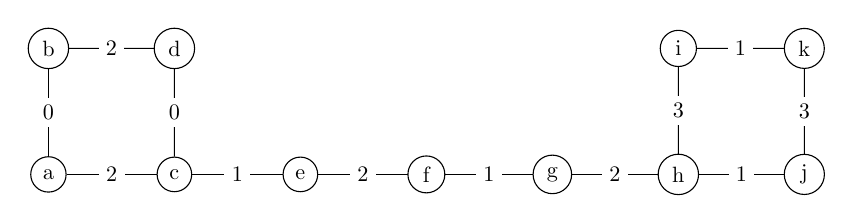
\begin{tikzpicture}[scale=.8]

        \begin{scope}[every node/.style={circle,draw, transform shape}]
          \node (1)  at (0,2)  {b};
          \node (2)  at (0,0)  {a};
          \node (3)  at (2,2)  {d};
          \node (4)  at (2,0)  {c};
          \node (5)  at (4,0)  {e};
          \node (6)  at (6,0)  {f};
          \node (7)  at (8,0)  {g};
          \node (8)  at (10,0) {h};
          \node (9)  at (10,2) {i};
          \node (10) at (12,0) {j};
          \node (11) at (12,2) {k};
        \end{scope}

        \begin{scope}[every node/.style={fill=white, transform shape}]

          \begin{scope}[every edge/.style={draw}]
            \path (1)  edge node {$0$} (2);
            \path (3)  edge node {$0$} (4);
            \path (4)  edge node {$1$} (5);
            \path (6)  edge node {$1$} (7);
            \path (8)  edge node {$1$} (10);
            \path (9)  edge node {$1$} (11);
            \path (1)  edge node {$2$} (3);
            \path (2)  edge node {$2$} (4);
            \path (5)  edge node {$2$} (6);
            \path (7)  edge node {$2$} (8);
            \path (8)  edge node {$3$} (9);
            \path (10) edge node {$3$} (11);
          \end{scope}
        \end{scope}

      \end{tikzpicture}
      \caption{}
    \end{center}
  \end{figure}

  \paragraph{}
  In both graphs, a $\rho_0$ edge can be placed on $(j,k)$ and a $\rho_3$ edge on $(a,b)$. In the first one, there is no possibility for the last $\rho_3$ edge. In the second graph the last $\rho_0$ edge must be placed on $(e,f)$ but the the last $\rho_3$ cannot be placed on $(f,g)$ and thus anywhere.

  \paragraph{}
  This concludes this part of the proof.

  \paragraph{}
  \textbf{One vertex shared}

  \paragraph{}
  If one vertex is shared, then a rotation pattern must be used between the two squares (see Proposition~\ref{rotation-pattern}).

  \begin{figure}[H]
    \begin{center}
      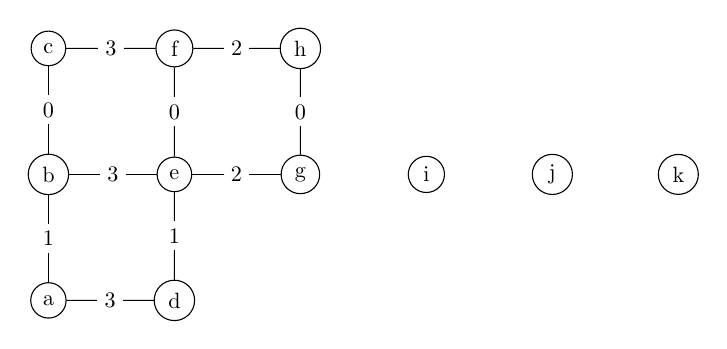
\begin{tikzpicture}[scale=.8]

        \begin{scope}[every node/.style={circle,draw, transform shape}]
          \node (1)  at (0,2)  {c};
          \node (2)  at (0,0)  {b};
          \node (3)  at (0,-2) {a};
          \node (4)  at (2,2)  {f};
          \node (5)  at (2,0)  {e};
          \node (6)  at (2,-2) {d};
          \node (7)  at (4,2)  {h};
          \node (8)  at (4,0)  {g};
          \node (9)  at (6,0)  {i};
          \node (10) at (8,0)  {j};
          \node (11) at (10,0) {k};
        \end{scope}

        \begin{scope}[every node/.style={fill=white, transform shape}]

          \begin{scope}[every edge/.style={draw}]
            \path (1)  edge node {$0$} (2);
            \path (4)  edge node {$0$} (5);
            \path (7)  edge node {$0$} (8);
            \path (2)  edge node {$1$} (3);
            \path (5)  edge node {$1$} (6);
            \path (4)  edge node {$2$} (7);
            \path (5)  edge node {$2$} (8);
            \path (1)  edge node {$3$} (4);
            \path (2)  edge node {$3$} (5);
            \path (3)  edge node {$3$} (6);
          \end{scope}
        \end{scope}

      \end{tikzpicture}
      \caption{}
    \end{center}
  \end{figure}

  \paragraph{}
  We need to place all the other patterns deduced from the usages of Lemma~\ref{rank-4-3-patterns}. The edges $(b,c)$ or $(c,f)$ can be used to form those patterns. First we suppose that both are single edges and then we examine the case where one of the edge is a double edge.

  \paragraph{}
  Both double edges cannot be placed on vertices $i,j,k$ because two double edges cannot be adjacent. Thus one double edge must share a vertex with an alternating square. Hence it must be inside this alternating square. Suppose that this edge is $(\rho_0, \rho_2)$ (using $(\rho_0, \rho_3)$ gives the same situation up to duality), it cannot use any other vertex already used by an edge $\rho_0$ or $\rho_2$. The only possibility is $(a,d)$. If the other double edge is placed in this component, it must be placed on $(g,h)$ but then this component cannot be connected to anything and thus the graph can not be connected.

  \paragraph{}
  Now the component $\{a,b,c,d,e,f,g,h\}$ can not be extended by $a$ or $b$. If it is extended on $g$ and $h$ then there are no more free vertices for the double edges $(\rho_1, \rho_3)$, and it must be placed on the big component, but this component cannot be extended by previous statement.

  \paragraph{}
  The double edge $(\rho_1, \rho_3)$ must be on the three remaining points. This edge must be connected to a $\rho_2$ edge. But this $\rho_2$ edge cannot have its other vertex in the big component.

  \begin{figure}[H]
    \begin{center}
      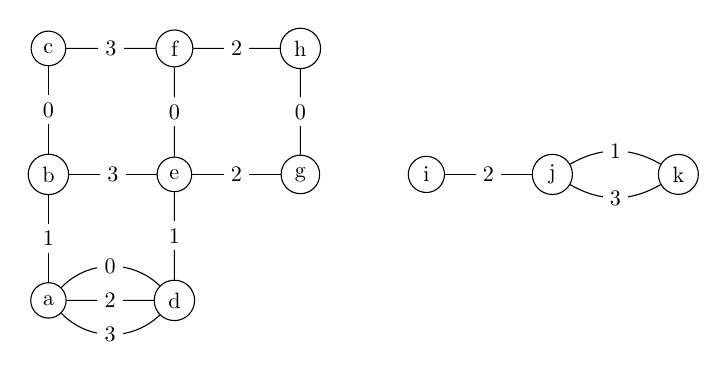
\begin{tikzpicture}[scale=.8]

        \begin{scope}[every node/.style={circle,draw, transform shape}]
          \node (1)  at (0,2)  {c};
          \node (2)  at (0,0)  {b};
          \node (3)  at (0,-2) {a};
          \node (4)  at (2,2)  {f};
          \node (5)  at (2,0)  {e};
          \node (6)  at (2,-2) {d};
          \node (7)  at (4,2)  {h};
          \node (8)  at (4,0)  {g};
          \node (9)  at (6,0)  {i};
          \node (10) at (8,0)  {j};
          \node (11) at (10,0) {k};
        \end{scope}

        \begin{scope}[every node/.style={fill=white, transform shape}]

          \begin{scope}[every edge/.style={draw}]
            \path (1)  edge node {$0$} (2);
            \path (3)  edge[bend left=45] node {$0$} (6);
            \path (4)  edge node {$0$} (5);
            \path (7)  edge node {$0$} (8);
            \path (2)  edge node {$1$} (3);
            \path (5)  edge node {$1$} (6);
            \path (10) edge[bend left=30] node {$1$} (11);
            \path (3)  edge node {$2$} (6);
            \path (4)  edge node {$2$} (7);
            \path (5)  edge node {$2$} (8);
            \path (9)  edge node {$2$} (10);
            \path (1)  edge node {$3$} (4);
            \path (2)  edge node {$3$} (5);
            \path (3)  edge[bend right=45] node {$3$} (6);
            \path (10) edge[bend right=30] node {$3$} (11);
          \end{scope}
        \end{scope}

      \end{tikzpicture}
      \caption{}
    \end{center}
  \end{figure}

  \paragraph{}
  Because the sequence of alternating squares cannot be extended, a single $\rho_1$ edge must connect either $g$ or $h$ to the fixed point $i$. That gives us two graphs:

  \begin{figure}[H]
    \begin{center}
      \begin{tikzpicture}[scale=.8]

        \begin{scope}[every node/.style={circle,draw, transform shape}]
          \node (1)  at (0,2)  {};
          \node (2)  at (0,0)  {};
          \node (3)  at (0,-2) {};
          \node (4)  at (2,2)  {};
          \node (5)  at (2,0)  {};
          \node (6)  at (2,-2) {};
          \node (7)  at (4,2)  {};
          \node (8)  at (4,0)  {};
          \node (9)  at (6,0)  {};
          \node (10) at (8,0)  {};
          \node (11) at (10,0) {};
        \end{scope}

        \begin{scope}[every node/.style={fill=white, transform shape}]

          \begin{scope}[every edge/.style={draw}]
            \path (1)  edge node {$0$} (2);
            \path (3)  edge[bend left=45] node {$0$} (6);
            \path (4)  edge node {$0$} (5);
            \path (7)  edge node {$0$} (8);
            \path (2)  edge node {$1$} (3);
            \path (5)  edge node {$1$} (6);
            \path (8)  edge node {$1$} (9);
            \path (10) edge[bend left=30] node {$1$} (11);
            \path (3)  edge node {$2$} (6);
            \path (4)  edge node {$2$} (7);
            \path (5)  edge node {$2$} (8);
            \path (9)  edge node {$2$} (10);
            \path (1)  edge node {$3$} (4);
            \path (2)  edge node {$3$} (5);
            \path (3)  edge[bend right=45] node {$3$} (6);
            \path (10) edge[bend right=30] node {$3$} (11);
          \end{scope}
        \end{scope}

      \end{tikzpicture}
      \caption{}
    \end{center}
  \end{figure}

  \begin{figure}[H]
    \begin{center}
      \begin{tikzpicture}[scale=.8]

        \begin{scope}[every node/.style={circle,draw, transform shape}]
          \node (1)  at (0,2)  {};
          \node (2)  at (0,0)  {};
          \node (3)  at (0,-2) {};
          \node (4)  at (2,2)  {};
          \node (5)  at (2,0)  {};
          \node (6)  at (2,-2) {};
          \node (7)  at (4,2)  {};
          \node (8)  at (4,0)  {};
          \node (9)  at (6,2)  {};
          \node (10) at (8,2)  {};
          \node (11) at (10,2) {};
        \end{scope}

        \begin{scope}[every node/.style={fill=white, transform shape}]

          \begin{scope}[every edge/.style={draw}]
            \path (1)  edge node {$0$} (2);
            \path (3)  edge[bend left=45] node {$0$} (6);
            \path (4)  edge node {$0$} (5);
            \path (7)  edge node {$0$} (8);
            \path (2)  edge node {$1$} (3);
            \path (5)  edge node {$1$} (6);
            \path (7)  edge node {$1$} (9);
            \path (10) edge[bend left=30] node {$1$} (11);
            \path (3)  edge node {$2$} (6);
            \path (4)  edge node {$2$} (7);
            \path (5)  edge node {$2$} (8);
            \path (9)  edge node {$2$} (10);
            \path (1)  edge node {$3$} (4);
            \path (2)  edge node {$3$} (5);
            \path (3)  edge[bend right=45] node {$3$} (6);
            \path (10) edge[bend right=30] node {$3$} (11);
          \end{scope}
        \end{scope}

      \end{tikzpicture}
      \caption{}
    \end{center}
  \end{figure}

  \paragraph{}
  Now we prove that both of those graphs are string C-group representations of $A_{11}$. To prove this, remove the $\rho_3$ edge. Both graphs become:

  \begin{figure}[H]
    \begin{center}
      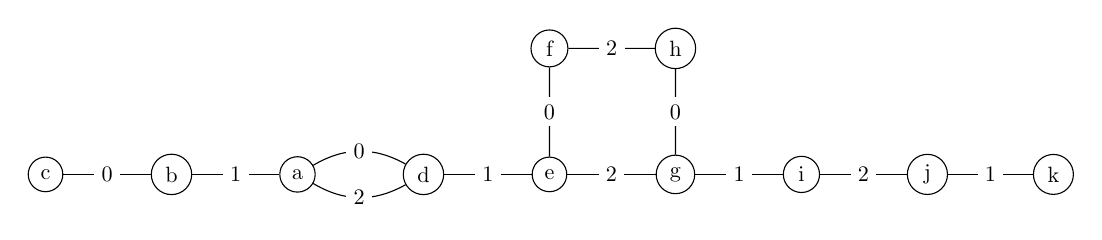
\begin{tikzpicture}[scale=.8]

        \begin{scope}[every node/.style={circle,draw, transform shape}]
          \node (1)  at (-6,0) {c};
          \node (2)  at (-4,0) {b};
          \node (3)  at (-2,0) {a};
          \node (4)  at (2,2)  {f};
          \node (5)  at (2,0)  {e};
          \node (6)  at (0,0)  {d};
          \node (7)  at (4,2)  {h};
          \node (8)  at (4,0)  {g};
          \node (9)  at (6,0)  {i};
          \node (10) at (8,0)  {j};
          \node (11) at (10,0) {k};
        \end{scope}

        \begin{scope}[every node/.style={fill=white, transform shape}]

          \begin{scope}[every edge/.style={draw}]
            \path (1)  edge node {$0$} (2);
            \path (3)  edge[bend left=30] node {$0$} (6);
            \path (4)  edge node {$0$} (5);
            \path (7)  edge node {$0$} (8);
            \path (2)  edge node {$1$} (3);
            \path (5)  edge node {$1$} (6);
            \path (8)  edge node {$1$} (9);
            \path (10) edge node {$1$} (11);
            \path (3)  edge[bend right=30] node {$2$} (6);
            \path (4)  edge node {$2$} (7);
            \path (5)  edge node {$2$} (8);
            \path (9)  edge node {$2$} (10);
          \end{scope}
        \end{scope}

      \end{tikzpicture}
      \caption{}
    \end{center}
  \end{figure}

  \begin{figure}[H]
    \begin{center}
      \begin{tikzpicture}[scale=.8]

        \begin{scope}[every node/.style={circle,draw, transform shape}]
          \node (1)  at (-6,0) {};
          \node (2)  at (-4,0) {};
          \node (3)  at (-2,0) {};
          \node (4)  at (2,2)  {};
          \node (5)  at (2,0)  {};
          \node (6)  at (0,0)  {};
          \node (7)  at (4,2)  {};
          \node (8)  at (4,0)  {};
          \node (9)  at (6,2)  {};
          \node (10) at (8,2)  {};
          \node (11) at (10,2) {};
        \end{scope}

        \begin{scope}[every node/.style={fill=white, transform shape}]

          \begin{scope}[every edge/.style={draw}]
            \path (1)  edge node {$0$} (2);
            \path (3)  edge[bend left=30] node {$0$} (6);
            \path (4)  edge node {$0$} (5);
            \path (7)  edge node {$0$} (8);
            \path (2)  edge node {$1$} (3);
            \path (5)  edge node {$1$} (6);
            \path (7)  edge node {$1$} (9);
            \path (10) edge node {$1$} (11);
            \path (3)  edge[bend right=30] node {$2$} (6);
            \path (4)  edge node {$2$} (7);
            \path (5)  edge node {$2$} (8);
            \path (9)  edge node {$2$} (10);
          \end{scope}
        \end{scope}

      \end{tikzpicture}
      \caption{}
    \end{center}
  \end{figure}

  \paragraph{}
  As usual, only the first case is proved and the other are left to the reader.

  \paragraph{}
  The group displayed is transitive because the graph is connected. Furthermore it is 2-transitive. To prove that, we must find permutations that keep $c$ fixed and that send $b$ to any other unfixed point. However $c$ keep fixed if no $\rho_0$ edge are used, thus $b$ can be easily send to $a,d,e,g,i,j,k$ while keeping $c$ fixed. Now we only need to find a permutation that sends $c$ fixed and that sends $b$ to $f$ or $h$. This permutation is $(\rho_1\rho_2)^3\rho_0\rho_1\rho_2\rho_0\rho_1\rho_0$.

  \paragraph{}
  The group is 2-transitive thus primitive. Its order is a multiple of $11 \times 10$ and of the order of the subgroups: $D_{12}$ and $D_{16}$. The order is thus a multiple of $11 \times 5 \times 3 \times 2^4 = 2640$. By looking at the primitive groups of degree 11 in~\cite{buekenhout1996list}, there are only three possible groups: $M_{11}$, $A_{11}$ and $S_{11}$. The first can be eliminated because $D_{16}$ is not one of its subgroup, $S_{11}$ contains odd permutations but the graph only contains even generators and thus cannot generate $S_{11}$.

  \paragraph{}
  The only solution is $A_{11}$. But if $\Gamma_{\rho_0, \rho_1, \rho_2} = \Gamma = A_{11}$, then $\Gamma$ cannot satisfy the intersection property by~\ref{not-monodromy-intersection}.

  \paragraph{}
  The last possibility is to move the double edge on $(c,d)$. The graph is this one:

  \begin{figure}[H]
    \begin{center}
      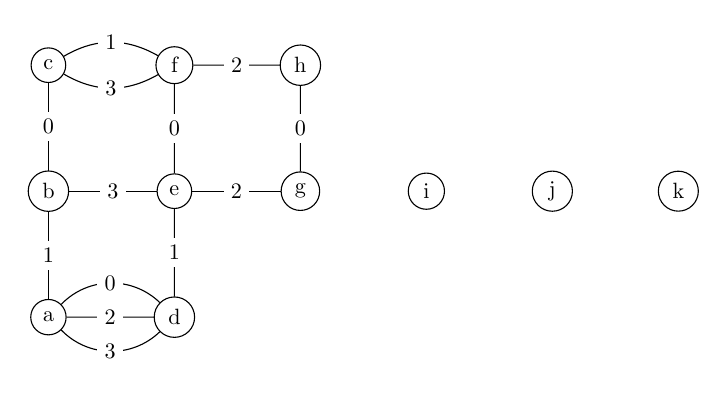
\begin{tikzpicture}[scale=.8]

        \begin{scope}[every node/.style={circle,draw, transform shape}]
          \node (1)  at (0,2)  {c};
          \node (2)  at (0,0)  {b};
          \node (3)  at (0,-2) {a};
          \node (4)  at (2,2)  {f};
          \node (5)  at (2,0)  {e};
          \node (6)  at (2,-2) {d};
          \node (7)  at (4,2)  {h};
          \node (8)  at (4,0)  {g};
          \node (9)  at (6,0)  {i};
          \node (10) at (8,0)  {j};
          \node (11) at (10,0) {k};
        \end{scope}

        \begin{scope}[every node/.style={fill=white, transform shape}]

          \begin{scope}[every edge/.style={draw}]
            \path (1)  edge node {$0$} (2);
            \path (3)  edge[bend left=45] node {$0$} (6);
            \path (4)  edge node {$0$} (5);
            \path (7)  edge node {$0$} (8);
            \path (2)  edge node {$1$} (3);
            \path (5)  edge node {$1$} (6);
            \path (1)  edge[bend left=30] node {$1$} (4);
            \path (3)  edge node {$2$} (6);
            \path (4)  edge node {$2$} (7);
            \path (5)  edge node {$2$} (8);
            \path (1)  edge[bend right=30] node {$3$} (4);
            \path (2)  edge node {$3$} (5);
            \path (3)  edge[bend right=45] node {$3$} (6);
          \end{scope}
        \end{scope}

      \end{tikzpicture}
      \caption{}
    \end{center}
  \end{figure}

  \paragraph{}
  There are 16 edges to link 11 vertices, thus we have 6 "joker" edges. We already built three alternating square and three double edges and thus all of them have been used. All new edges must link two different components.

  \paragraph{}
  The big component can only be linked by a $\rho_1$ edge from $g$ or $h$. Then there are a remaining $\rho_2$ edge and a remaining $\rho_3$ edge and thus the possible graphs are:

  \begin{figure}[H]
    \begin{center}
      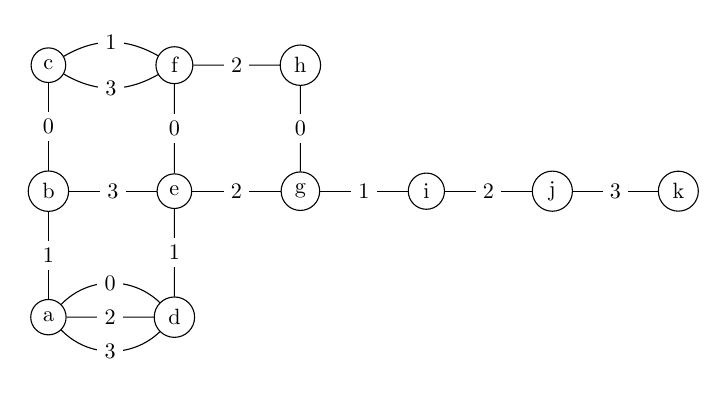
\begin{tikzpicture}[scale=.8]

        \begin{scope}[every node/.style={circle,draw, transform shape}]
          \node (1)  at (0,2)  {c};
          \node (2)  at (0,0)  {b};
          \node (3)  at (0,-2) {a};
          \node (4)  at (2,2)  {f};
          \node (5)  at (2,0)  {e};
          \node (6)  at (2,-2) {d};
          \node (7)  at (4,2)  {h};
          \node (8)  at (4,0)  {g};
          \node (9)  at (6,0)  {i};
          \node (10) at (8,0)  {j};
          \node (11) at (10,0) {k};
        \end{scope}

        \begin{scope}[every node/.style={fill=white, transform shape}]

          \begin{scope}[every edge/.style={draw}]
            \path (1)  edge node {$0$} (2);
            \path (3)  edge[bend left=45] node {$0$} (6);
            \path (4)  edge node {$0$} (5);
            \path (7)  edge node {$0$} (8);
            \path (2)  edge node {$1$} (3);
            \path (5)  edge node {$1$} (6);
            \path (8)  edge node {$1$} (9);
            \path (1)  edge[bend left=30] node {$1$} (4);
            \path (3)  edge node {$2$} (6);
            \path (4)  edge node {$2$} (7);
            \path (5)  edge node {$2$} (8);
            \path (9)  edge node {$2$} (10);
            \path (1)  edge[bend right=30] node {$3$} (4);
            \path (2)  edge node {$3$} (5);
            \path (3)  edge[bend right=45] node {$3$} (6);
            \path (10) edge node {$3$} (11);
          \end{scope}
        \end{scope}

      \end{tikzpicture}
      \caption{}
    \end{center}
  \end{figure}

  \begin{figure}[H]
    \begin{center}
      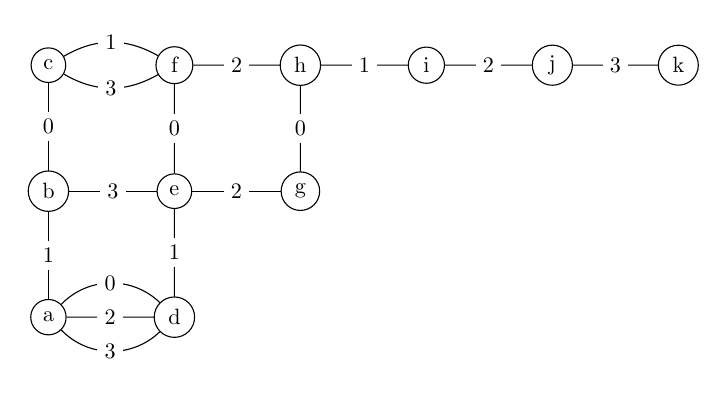
\begin{tikzpicture}[scale=.8]

        \begin{scope}[every node/.style={circle,draw, transform shape}]
          \node (1)  at (0,2)  {c};
          \node (2)  at (0,0)  {b};
          \node (3)  at (0,-2) {a};
          \node (4)  at (2,2)  {f};
          \node (5)  at (2,0)  {e};
          \node (6)  at (2,-2) {d};
          \node (7)  at (4,2)  {h};
          \node (8)  at (4,0)  {g};
          \node (9)  at (6,2)  {i};
          \node (10) at (8,2)  {j};
          \node (11) at (10,2) {k};
        \end{scope}

        \begin{scope}[every node/.style={fill=white, transform shape}]

          \begin{scope}[every edge/.style={draw}]
            \path (1)  edge node {$0$} (2);
            \path (3)  edge[bend left=45] node {$0$} (6);
            \path (4)  edge node {$0$} (5);
            \path (7)  edge node {$0$} (8);
            \path (2)  edge node {$1$} (3);
            \path (5)  edge node {$1$} (6);
            \path (7)  edge node {$1$} (9);
            \path (1)  edge[bend left=30] node {$1$} (4);
            \path (3)  edge node {$2$} (6);
            \path (4)  edge node {$2$} (7);
            \path (5)  edge node {$2$} (8);
            \path (9)  edge node {$2$} (10);
            \path (1)  edge[bend right=30] node {$3$} (4);
            \path (2)  edge node {$3$} (5);
            \path (3)  edge[bend right=45] node {$3$} (6);
            \path (10) edge node {$3$} (11);
          \end{scope}
        \end{scope}

      \end{tikzpicture}
      \caption{}
    \end{center}
  \end{figure}

  \paragraph{}
  However the group generated by the last graph is not $A_{11}$ but $\PSL_2(11)$ which is of order 660. This can easily be checked by the reader using Property~\ref{orbit-stabilizer}.

  \paragraph{}
  Thus the monodromy group generating $A_{11}$ is the group displayed in the first graph.

\end{proof}

\begin{lemma}
  \label{proof-4-2}
  This monodromy group is not a string C-group representation of $A_{11}$.
\end{lemma}

\begin{proof}
  As in previous sections, the proof of this statement is left to the reader.
\end{proof}

\paragraph{}
Now we can summarized what we have seen in Lemmas~\ref{proof-2-1}, \ref{proof-2-2}, \ref{proof-3-1}, \ref{proof-3-2}, \ref{proof-4-1} and~\ref{proof-4-2}:

\begin{theorem}
  There does not exist a string C-group representation of rank 4 of $A_{11}$.
\end{theorem}
